\section{Resultados}

\subsection{Controles negativos}

Se realizaron tres experimentos de 72\,h los días 20260404, 20260428 y 20260507, para un total de \(n = 81\) bandejas (27 por día). La variable principal de análisis fue el \textbf{cambio porcentual de peso} (\emph{pct\_change} en el código de análisis), definido como el aumento de masa respecto al peso inicial de las semillas en cada bandeja. Como verificación de robustez, los principales análisis se repitieron con dos variables de crecimiento alternativas: el \textbf{cambio absoluto de peso} (\emph{raw\_delta\_weight}), definido como la diferencia entre el peso final e inicial en gramos, y el \textbf{logaritmo de la razón de pesos} (\emph{raw\_log\_ratio}), definido como el logaritmo natural del cociente entre el peso final y el inicial. Estas tres variables cuantifican el mismo fenómeno de crecimiento con distintas propiedades estadísticas; su coincidencia en dirección y significancia refuerza que los efectos reportados no dependen de la métrica elegida.

\subsubsection{Supuestos estadísticos}

Se evaluó la normalidad de los residuos mediante el test de Shapiro-Wilk y la homogeneidad de varianzas mediante el test de Brown-Forsythe. Para el cambio porcentual de peso, los residuos resultaron normales (\(p = 0.5773\)) pero las varianzas no resultaron homogéneas entre días (\(p = 0.0302\)). Por lo tanto, los modelos presentados a continuación fueron ajustados por día experimental y utilizan errores robustos HC3 para compensar la heterogeneidad de varianzas.

\subsubsection{Calidad del armado (pesos iniciales)}

Para descartar un posible sesgo de selección al momento de armar las bandejas, se analizó si las semillas iniciales tenían masas diferentes entre pisos. El resultado no fue significativo (\(p = 0.4926\)), lo que indica que los pisos A, B y C comenzaron con masas de semillas estadísticamente equivalentes. Las diferencias observadas al final del experimento se atribuyen, por lo tanto, a factores ocurridos durante el crecimiento y no a un sesgo inicial.

\subsubsection{Efecto del piso (A, B, C)}

La Figura~\ref{fig:ctrl_pct_change_floor} muestra el crecimiento relativo promedio para cada piso. La Tabla~\ref{tab:ctrl_floor} presenta las medias y desvíos estándar.

\begin{table}[h]
\centering
\caption{Crecimiento relativo (cambio porcentual de peso) por piso en controles negativos combinados. Los valores se expresan como media \(\pm\) SD entre bandejas dentro de cada grupo (\(n = 27\) por piso).}
\label{tab:ctrl_floor}
\begin{tabular}{lc}
\hline
Piso & Media \(\pm\) SD \\
\hline
A & 0.4455 \(\pm\) 0.0376 \\
B & 0.4261 \(\pm\) 0.0448 \\
C & 0.4094 \(\pm\) 0.0534 \\
\hline
\end{tabular}
\end{table}

Se observaron diferencias significativas entre pisos (\(F_{2,76} = 3.9746\), \(p = 0.0228\)), con un patrón consistente A \(>\) B \(>\) C en crecimiento promedio.

Como verificación de robustez, el mismo análisis se repitió utilizando el cambio absoluto de peso y el logaritmo de la razón de pesos. La Tabla~\ref{tab:ctrl_floor_robustez} presenta las medias y desvíos estándar por piso para ambas variables, junto con los resultados del test de diferencias.

\begin{table}[h]
\centering
\caption{Crecimiento por piso para el cambio absoluto de peso y el logaritmo de la razón de pesos, como verificación de robustez del efecto observado con el cambio porcentual de peso. Los valores se expresan como media \(\pm\) SD entre bandejas dentro de cada grupo (\(n = 27\) por piso).}
\label{tab:ctrl_floor_robustez}
\begin{tabular}{lcccc}
\hline
Variable & Piso A & Piso B & Piso C & \(F_{2,76}\) (\(p\)) \\
\hline
Cambio absoluto de peso & 1.6412 \(\pm\) 0.1463 & 1.5860 \(\pm\) 0.1796 & 1.4892 \(\pm\) 0.1964 & 4.7870 (0.0110) \\
Logaritmo razón de pesos & 0.3681 \(\pm\) 0.0261 & 0.3545 \(\pm\) 0.0314 & 0.3425 \(\pm\) 0.0378 & 4.0686 (0.0210) \\
\hline
\end{tabular}
\end{table}

Ambas variables reproducen el mismo patrón A \(>\) B \(>\) C y alcanzan significancia estadística, confirmando que el efecto de piso no depende de la métrica de crecimiento elegida. Adicionalmente, se verificó el resultado mediante un ANOVA clásico ajustado por día experimental (sin errores robustos), obteniéndose resultados consistentes para las tres variables (Tabla~\ref{tab:ctrl_floor_anova_clasico}).

\begin{table}[h]
\centering
\caption{Verificación del efecto de piso mediante ANOVA clásico ajustado por día experimental.}
\label{tab:ctrl_floor_anova_clasico}
\begin{tabular}{lcc}
\hline
Variable & \(F\) clásico & \(p\) clásico \\
\hline
Cambio absoluto de peso & 5.1563 & 0.00794 \\
Cambio porcentual de peso & 4.2663 & 0.0175 \\
Logaritmo razón de pesos  & 4.3650 & 0.0161 \\
\hline
\end{tabular}
\end{table}

\begin{figure}[H]
    \centering
    \includegraphics[width=0.75\linewidth]{datos/software_data/analysis/negative_control_combined/negative_control_combined_pct_change_floor_barplot.png}
    \caption{Crecimiento relativo (cambio porcentual de peso) por piso en controles negativos combinados. Cada punto corresponde a una bandeja individual, coloreada según el día del experimento.}
    \label{fig:ctrl_pct_change_floor}
\end{figure}

\subsubsection{Efecto de la posición lateral (izquierda, centro, derecha)}

La Figura~\ref{fig:ctrl_pct_change_lcr} muestra el crecimiento según la posición lateral. La Tabla~\ref{tab:ctrl_lcr} presenta los valores numéricos.

\begin{table}[h]
\centering
\caption{Crecimiento relativo (cambio porcentual de peso) según posición lateral. Izquierda = celdas 1, 4, 7; centro = 2, 5, 8; derecha = 3, 6, 9. \(n = 27\) por grupo.}
\label{tab:ctrl_lcr}
\begin{tabular}{lc}
\hline
Posición & Media \(\pm\) SD \\
\hline
Izquierda & 0.4176 \(\pm\) 0.0465 \\
Centro    & 0.4264 \(\pm\) 0.0498 \\
Derecha   & 0.4370 \(\pm\) 0.0460 \\
\hline
\end{tabular}
\end{table}

No se detectaron diferencias significativas entre izquierda, centro y derecha (\(F_{2,76} = 1.1339\), \(p = 0.3272\)).

El mismo análisis con el cambio absoluto de peso y el logaritmo de la razón de pesos confirma la ausencia de efecto lateral (Tabla~\ref{tab:ctrl_lcr_robustez}).

\begin{table}[h]
\centering
\caption{Crecimiento según posición lateral para el cambio absoluto de peso y el logaritmo de la razón de pesos, como verificación de robustez. \(n = 27\) por grupo.}
\label{tab:ctrl_lcr_robustez}
\begin{tabular}{lcccc}
\hline
Variable & Izquierda & Centro & Derecha & \(F_{2,76}\) (\(p\)) \\
\hline
Cambio absoluto de peso & 1.5506 \(\pm\) 0.1754 & 1.5726 \(\pm\) 0.2022 & 1.5932 \(\pm\) 0.1787 & 0.3598 (0.6990) \\
Logaritmo razón de pesos & 0.3484 \(\pm\) 0.0331 & 0.3546 \(\pm\) 0.0348 & 0.3621 \(\pm\) 0.0322 & 1.1254 (0.3299) \\
\hline
\end{tabular}
\end{table}

\begin{figure}[H]
    \centering
    \includegraphics[width=0.75\linewidth]{datos/software_data/analysis/negative_control_combined/negative_control_combined_pct_change_left_center_right_barplot.png}
    \caption{Crecimiento relativo (cambio porcentual de peso) según posición lateral (izquierda, centro, derecha) en controles negativos combinados.}
    \label{fig:ctrl_pct_change_lcr}
\end{figure}

\subsubsection{Efecto de la profundidad (frente, medio, atrás)}

La Figura~\ref{fig:ctrl_pct_change_fmb} muestra el crecimiento según la profundidad. La Tabla~\ref{tab:ctrl_fmb} presenta los valores.

\begin{table}[h]
\centering
\caption{Crecimiento relativo (cambio porcentual de peso) según profundidad. Frente = celdas 7, 8, 9; medio = 4, 5, 6; atrás = 1, 2, 3. \(n = 27\) por grupo.}
\label{tab:ctrl_fmb}
\begin{tabular}{lc}
\hline
Posición & Media \(\pm\) SD \\
\hline
Frente & 0.4170 \(\pm\) 0.0472 \\
Medio  & 0.4317 \(\pm\) 0.0554 \\
Atrás  & 0.4323 \(\pm\) 0.0388 \\
\hline
\end{tabular}
\end{table}

No se detectaron diferencias significativas entre frente, medio y atrás (\(F_{2,76} = 0.9012\), \(p = 0.4104\)).

El mismo análisis con el cambio absoluto de peso y el logaritmo de la razón de pesos confirma la ausencia de efecto de profundidad (Tabla~\ref{tab:ctrl_fmb_robustez}).

\begin{table}[h]
\centering
\caption{Crecimiento según profundidad para el cambio absoluto de peso y el logaritmo de la razón de pesos, como verificación de robustez. \(n = 27\) por grupo.}
\label{tab:ctrl_fmb_robustez}
\begin{tabular}{lcccc}
\hline
Variable & Frente & Medio & Atrás & \(F_{2,76}\) (\(p\)) \\
\hline
Cambio absoluto de peso & 1.5364 \(\pm\) 0.1561 & 1.5692 \(\pm\) 0.2369 & 1.6108 \(\pm\) 0.1454 & 1.5663 (0.2155) \\
Logaritmo razón de pesos & 0.3480 \(\pm\) 0.0336 & 0.3581 \(\pm\) 0.0387 & 0.3589 \(\pm\) 0.0272 & 0.9039 (0.4093) \\
\hline
\end{tabular}
\end{table}

\begin{figure}[H]
    \centering
    \includegraphics[width=0.75\linewidth]{datos/software_data/analysis/negative_control_combined/negative_control_combined_pct_change_front_middle_back_barplot.png}
    \caption{Crecimiento relativo (cambio porcentual de peso) según profundidad (frente, medio, atrás) en controles negativos combinados.}
    \label{fig:ctrl_pct_change_fmb}
\end{figure}

\subsubsection{Comparación entre todas las celdas (A1--C9)}

El análisis a escala de celda individual reveló diferencias significativas entre posiciones (\(F_{26,52} = 6.2658\), \(p = 1.07 \times 10^{-8}\)). El mismo análisis, realizado con el cambio absoluto de peso (\(F_{26,52} = 6.2815\), \(p = 1.03 \times 10^{-8}\)) y con el logaritmo de la razón de pesos (\(F_{26,52} = 6.5493\), \(p = 5.04 \times 10^{-9}\)), confirma la existencia de un efecto de celda independientemente de la métrica de crecimiento utilizada.

La Figura~\ref{fig:ctrl_pct_change_heatmap} presenta un mapa de calor con el crecimiento relativo promedio de cada celda, permitiendo visualizar simultáneamente el patrón por piso y las diferencias finas entre celdas individuales.

\begin{figure}[H]
    \centering
    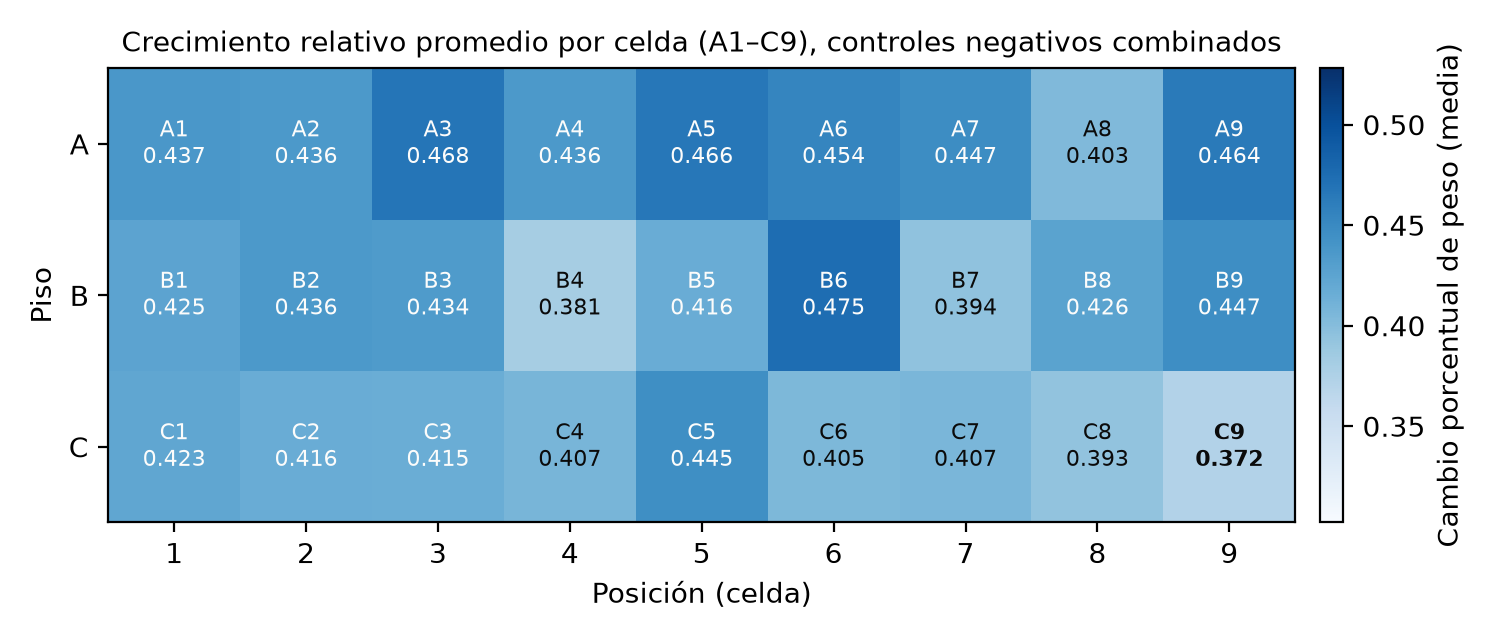
\includegraphics[width=0.85\linewidth]{datos/img/ctrl_pct_change_heatmap.png}
    \caption{Mapa de calor del crecimiento relativo promedio (cambio porcentual de peso) por celda (A1--C9) en controles negativos combinados. La celda C9 se destaca por presentar el menor valor promedio del conjunto.}
    \label{fig:ctrl_pct_change_heatmap}
\end{figure}

El análisis post-hoc por pares con corrección FDR identificó que las diferencias estuvieron principalmente asociadas a la celda C9, que presentó menor crecimiento relativo que varias celdas (Tabla~\ref{tab:ctrl_posthoc}).

\begin{table}[h]
\centering
\caption{Comparaciones post-hoc significativas (FDR) para el cambio porcentual de peso en el análisis A1--C9. Cada celda tiene \(n = 3\).}
\label{tab:ctrl_posthoc}
\begin{tabular}{lccc}
\hline
Comparación & Media celda 1 & Media celda 2 & Diferencia \\
\hline
C9 vs B8 & 0.3721 & 0.4263 & 0.0542 \\
C9 vs A1 & 0.3721 & 0.4373 & 0.0652 \\
C9 vs A9 & 0.3721 & 0.4636 & 0.0915 \\
C9 vs A3 & 0.3721 & 0.4676 & 0.0955 \\
C9 vs B6 & 0.3721 & 0.4751 & 0.1030 \\
\hline
\end{tabular}
\end{table}

Notar que si bien C9 presentó una desviación estándar muy pequeña (0.0114), esto refleja la consistencia entre las tres réplicas, no necesariamente una mayor precisión a nivel poblacional.

\begin{figure}[H]
    \centering
    \includegraphics[width=\linewidth]{datos/software_data/analysis/negative_control_combined/negative_control_combined_pct_change_tray_cell_barplot.png}
    \caption{Crecimiento relativo (cambio porcentual de peso) por celda individual (A1--C9) en controles negativos combinados. Se observa el menor crecimiento relativo de la celda C9 respecto de las demás.}
    \label{fig:ctrl_pct_change_all}
\end{figure}

\subsubsection{Conclusión parcial}

En los controles negativos combinados se detectó un efecto espacial general asociado al piso de la bandeja (A \(>\) B \(>\) C), pero no a los ejes izquierda-centro-derecha ni frente-medio-atrás. Sin embargo, al analizar cada celda individual A1--C9, se observaron diferencias significativas entre posiciones específicas. El análisis post-hoc indicó que estas diferencias estuvieron principalmente asociadas a la celda C9, que presentó menor crecimiento relativo que varias celdas de mayor crecimiento. Esto sugiere que el control negativo no fue completamente homogéneo a escala espacial fina, por lo que los análisis de tratamientos deberían considerar o controlar posibles efectos de posición.
